\chapter{Weather Balloon}
\label{chap:WB}
In this chapter we'll infer optical information about the ice the detectors reside in
using radio signals coming from a weather balloon flying over the stations. 

Every day in the summer, 2 times a day, a weather balloon gets launched
from base camp at Summit in Greenland. This weather balloon has an antenna
strapped to it constantly emitting a sinusoidal signal of 0.403GHz.

We can use this signal to find the index of refraction locally at the phased
array.  We'll go about this by first finding the difference in timing between
channels by fitting the balloon's sinusoidal signal to the data, and then doing
a plane wave reconstruction, using the balloon angle in the reconstruction, 
with that finding the local index of refraction.  This procedure will
be explained more in depth over the following sections.

Prior to the measurements we'll need to be able to predict how accurate our
findings will be, for this we'll need to run a simulation with the hybrid ray
tracer (explained in chapter \ref{chapter:hybrid}).  
There is one change that needs to happen first to our algorithm for us
to be able to simulate this: The air observer has to be removed as to make a
ray tracing possible from within the air into the ice and onto the detector\cite{hybrid}.

\section{Plane Wave Reconstruction}
We want to do a plane wave reconstruction of the balloon's position as this
will make us able to infer the index of refraction between chosen channels.
Example paths the weather balloon produce that end up in the deep channels is
shown in figure \ref{fig:Example trajectory}, here the balloon emits a signal
which propagates straight in the air and then refracts in the ice. Locally in
the ice we can assume the wave to come in as a plane wave.
\begin{figure}
	\centering
	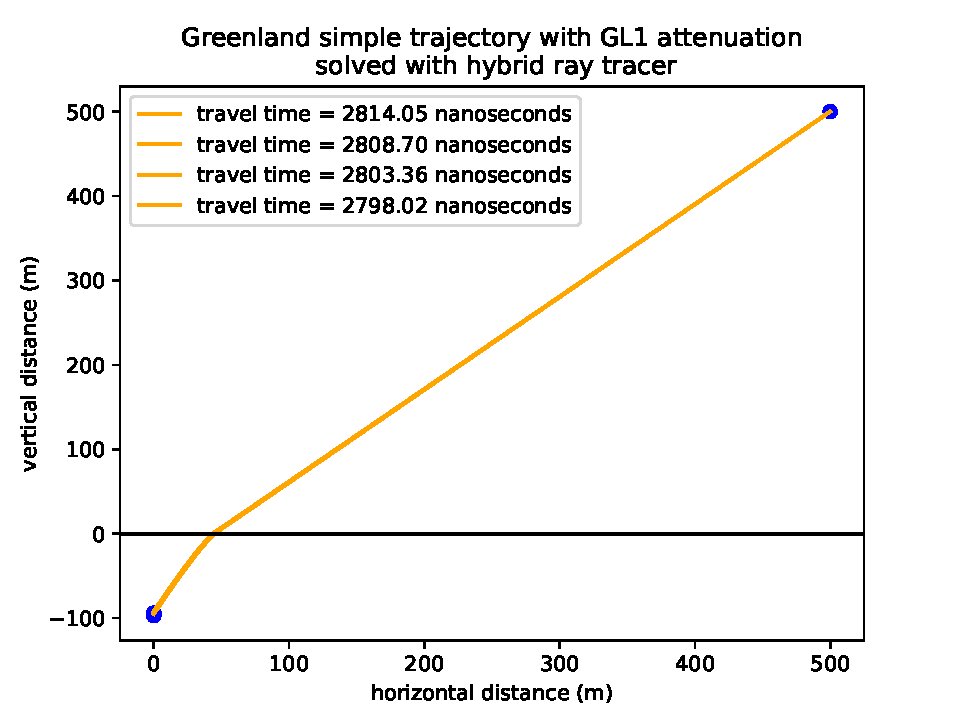
\includegraphics[width=0.7\textwidth]{weerballontraject.pdf}
	\caption{Example trajectory of rays coming from a weather balloon (red top right dot) and going through the ice to the various detectors (blue dots bottom left)}
	\label{fig:Example trajectory}
\end{figure}
\begin{figure}
	\centering
	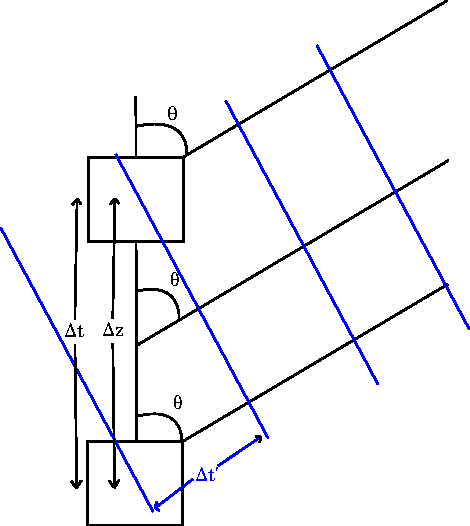
\includegraphics[width=0.7\textwidth]{planewave.pdf}
	\caption{The incoming signal can locally be seen as a plane wave, here drawn in blue. The channels are drawn in grey but are assumed to be points located at the center.}	
	\label{fig:Plane Wave}
\end{figure}

The arriving plane wave is shown as parallel lines in blue on figure \ref{fig:Plane Wave}. The
plane wave reconstruction method can be understood by taking a closer look at this figure, 
the radio waves coming from the weather balloon make a certain zenith angle $\theta$ with the detectors. The top detector (top box)
detects the wave at a certain time $t_1$, the bottom detector detects it at a
time $t_2$. After deciphering the data RNO-G recorded we'd thus see that these
two detectors got a signal $\Delta t = t_1 - t_2$ seconds apart from each other.
Now ideally this observed time is equal to the time it would theoretically take a plane
wave to propagate that distance ($\Delta t'$) which we can calculate from the geometry of
the problem and dimensional analysis:
\begin{equation}
	\Delta t' = \frac{m}{(m/s)} = (s/m)*m = v^{-1} * m = v^{-1} \cos\theta \Delta z
	\label{eqn:deltataccent}
\end{equation}
With $v = c/n$ the local speed of light, n the index of refraction at the depth in between
the considered channels and $\Delta z$ the distance between the channels. 
Thus if we know the zenith angle $\theta$, the difference in timing $\Delta t'$ and the distance between the channels $\Delta z$
we could infer the index of refraction at a certain depth as can be seen by reforming equation \ref{eqn:deltataccent}:
\begin{equation}
	n = \frac{\Delta t'}{\Delta z} \frac{c}{\cos\theta}
\end{equation}
We can actually roughly guess the angle, as for a balloon flying close to the
detector the incoming plane wave angle will be roughly the same as the angle the balloon
makes with the pair of channels ($\theta\approx\theta_b$).
At the actual index of refraction we thus expect the following function to show a 
minimum (go to zero):
\begin{equation}
	\eta(\theta,n) := (\Delta t - \Delta t') = \left(\Delta t
	- n\frac{\cos\theta_b \Delta z}{c}\right)
  	\label{eqn:eta}
\end{equation}
If we want to determine the index of refraction, 
we thus need to minimize equation \ref{eqn:eta}.

If we want to use more than 2 detectors at once however (which we'll
do for the phased array), we'll need to specify various functions to
minimize.  E.g if we have four detectors labeled 0 to 3 we'll have
to construct functions between detectors 0\&1, 0\&2, 0\&3, 1\&2,
1\&3 and 2\&3 . The further apart the detectors lie the larger the
function values and thus the more they will weigh in the sum. This importance to
further spaced channels is what we want as these will yield a more
accurate result. 
\subsection{simple plane wave reconstruction}
\label{seq:SimplePW}
To take into account all the different channels we take the sum of the
various eta functions (as defined in equation \ref{eqn:eta}) and
thus minimize the following function with respect the the index:
\begin{equation}
	f(n) := \sum_{i=\text{channel pairs}}\eta_i(n) = \sum_{i=\text{channel pairs}}\left( \Delta t_i - \frac{n\cos\theta_b \Delta z_i}{c}\right) \equiv \sum_{i<j}\left( \Delta t_{ij} - \frac{n\cos\theta_b \Delta z_{ij}}{c}\right)
  	\label{eqn:PlaneWave}
\end{equation}
where $\Delta t_{ij}$ denotes the observed time difference between
channels i and j, similarly $\Delta z_{ij}$ denotes the distance
between channels i and j.
If this function $f$ gets minimized, the n leading up to this minimzation
will be the answer we are seaking: the index of refraction inbetween
the various detectors.  
We now want to find the error on the index we fitted this way. To find the error on our result we need an expression for the index, let's solve for n:
\begin{align}
	f(n) &= \sum_{i<j}\left( \Delta t_{ij} - \frac{n\cos\theta_b \Delta z_{ij}}{c}\right)\\
\sum_{i<j}\frac{n\cos\theta_b \Delta z_{ij}}{c}&=\sum_{i<j}\Delta t_{ij} - f(n)\\
	n &= \frac{c}{\cos\theta_b}\left(\frac{\sum_{i<j}\Delta t_{ij}}{\sum_{i<j} \Delta z_{ij}} - \frac{f(n)}{\sum_{i<j} \Delta z_{ij}}\right)
\end{align}
Let's assume an error on the difference in propagation time between channel i and j
($\Delta t_{ij}$) of $\delta t_{ij}$, which we'll find out later.  For the
positional accuracy we'll assume to know the detector location to within 1cm\footnote{this
is a reasonable estimate as this is the accuracy of the reported channel positions},
this will imply an accuracy on $\Delta z_{ij}$ of 2cm.

Let's now compute the error on our predicted index:
\begin{align}
  \delta n &= \frac{c}{\cos{\theta_b}}\delta\left(\frac{\sum_{i<j}\Delta t_{ij}}{\sum_{i<j} \Delta z_{ij}} - \frac{f(n)}{\sum_{i<j} \Delta z_{ij}}\right)\\
  \delta n &= \frac{c}{\cos{\theta_b}}\delta\left(\frac{\sum_{i<j}\Delta t_{ij}}{\sum_{i<j} \Delta z_{ij}}\right)+ f(n)\frac{c}{\cos{\theta_b}}\delta\left(\frac{1}{\sum_{i<j} \Delta z_{ij}}\right)\\
\end{align}
Note here the function $\delta$ denotes the absolute error, let's define the function $RE$ to be the relative error and look at the terms individually:
\begin{align}
  \delta\left(\frac{\sum_{i<j}\Delta t_{ij}}{\sum_{i<j} \Delta z_{ij}}\right) &= \left(\frac{\sum_{i<j}\Delta t_{ij}}{\sum_{i<j} \Delta z_{ij}}\right)\times\left(RE\left(\sum_{i<j}\Delta t_{ij}\right) + RE\left(\sum_{i<j} \Delta z_{ij}\right)\right)\\
\delta\left(\frac{\sum_{i<j}\Delta t_{ij}}{\sum_{i<j} \Delta z_{ij}}\right) &= \left(\frac{\sum_{i<j}\Delta t_{ij}}{\sum_{i<j} \Delta z_{ij}}\right)\times\left(\frac{\sum_{i<j}\delta t_{ij}}{\sum_{i<j}\Delta t_{ij}} + \frac{\sum_{i<j}\delta z_{ij}}{\sum_{i<j}\Delta z_{ij}}\right)\\
\delta\left(\frac{\sum_{i<j}\Delta t_{ij}}{\sum_{i<j} \Delta z_{ij}}\right) &\approx \left(\frac{\sum_{i<j}\Delta t_{ij}}{\sum_{i<j} \Delta z_{ij}}\right)\times\left(\frac{\sum_{i<j}\delta t_{ij}}{\sum_{i<j}\Delta t_{ij}} + \frac{\sum_{i<j}0.02m}{\sum_{i<j}\Delta z_{ij}}\right) \delequal E_1\\
\end{align}
And now the second term:
\begin{align}
  \delta\left(\frac{1}{\sum_{i<j} \Delta z_{ij}}\right) &= \left(\frac{1}{\sum_{i<j} \Delta z_{ij}}\right)\times RE\left(\sum_{i<j}\Delta z_{ij}\right) \\
  \delta\left(\frac{1}{\sum_{i<j} \Delta z_{ij}}\right) &= \left(\frac{1}{\sum_{i<j} \Delta z_{ij}}\right)\times \frac{\delta\left(\sum_{i<j}\Delta z_{ij}\right)}{\sum_{i<j}\Delta z_{ij}} \\
  \delta\left(\frac{1}{\sum_{i<j} \Delta z_{ij}}\right) &= \frac{\sum_{i<j}\delta z_{ij}}{\left(\sum_{i<j}\Delta z_{ij}\right)^2} \\
  \delta\left(\frac{1}{\sum_{i<j} \Delta z_{ij}}\right) &\approx \frac{\sum_{i<j}0.02m}{\left(\sum_{i<j}\Delta z_{ij}\right)^2} \delequal E_2\\
\end{align}
So, finally:
\begin{align}
  \delta n &\approx \frac{c}{\cos\theta_b}\left(E_1 + f(n)E_2\right)
\end{align}
\subsection{plane wave reconstruction using snell's law}
\label{seq:SnellPW}
This was one way of fitting the index of refraction, another procedure
that we could do is by implementing breaking of the plane wave at 
the surface. 

We thus assume the reconstructed plane wave to behave like an actual wave
and, encountering the ice-air boundary, refracting according to snell's law.
This is useful for when the angle with the balloon is quite big as is illustrated
in figure \ref{fig:WeatherBalloonPositionReconstruction}, here you can clearly
see that, even though the plane wave locally matches the incoming signal, it
ends up really far away from the balloon. The reconstructed plane wave follows the
wave path closely until the air-ice boundary where the wave path got refracted,
we thus try doing the same thing by making the plane wave refract as well.

To find the index of refraction this way we can't minimize by taking the
incoming plane wave to have the same angle as the balloon, we'll need to look
at the distance between the plane wave reconstructed ray (after also refracting
at the surface) and the balloon, both at the height of the balloon.  The full
procedure then goes as follows: We first choose a certain index of refraction n, 
then we reconstruct the plane wave launch angle by minimizing the following function in
terms of $\theta$:
\begin{equation}
	f(\theta) := \sum_{i=\text{channel pairs}}\left( \Delta t_i - \frac{n\cos\theta \Delta z_i}{c}\right) \equiv \sum_{i<j}\left( \Delta t_{ij} - \frac{n\cos\theta \Delta z_{ij}}{c}\right)\label{eqn:snellmin}
\end{equation}
\begin{figure}
	\centering
	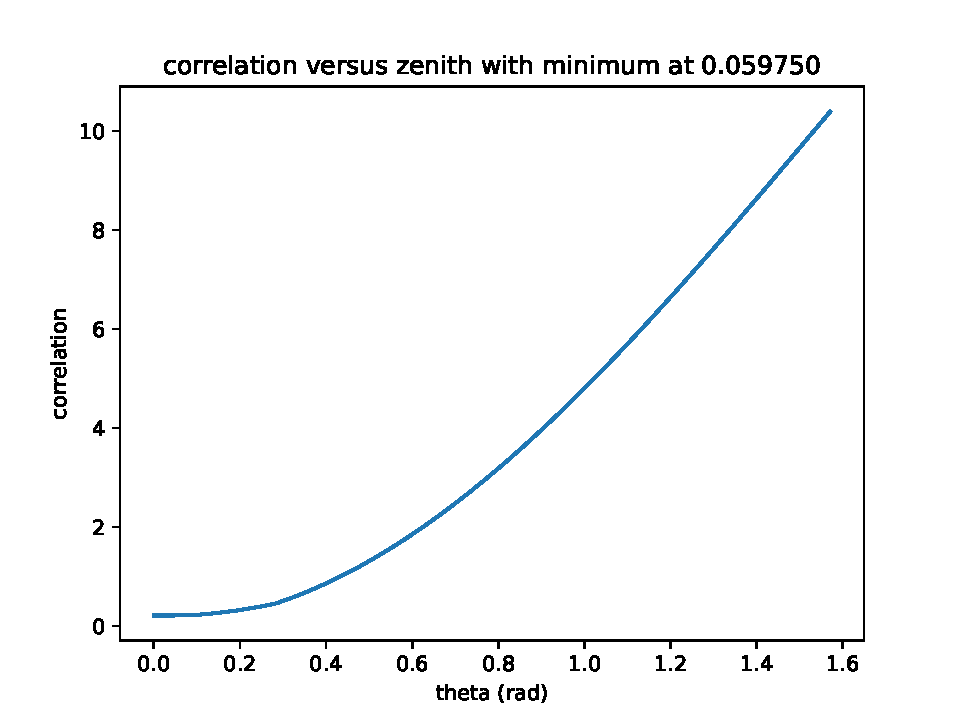
\includegraphics[width=0.8\textwidth]{SummedCorrelation.pdf}
	\caption{Example sum of the normed correlation functions}
	\label{fig:SummedCorrelation}
\end{figure}
Such a function is illustrated in figure \ref{fig:SummedCorrelation}.  For this
figure the modified hybrid ray tracing algorithm was used to simulate what the
difference in timing would be. 
As can be seen on the figure this function is minimal at a certain launch angle
$\theta_1$, we can use this angle and the height of the middle of the concerned
detectors to derive the path in the ice until it encounters the air-ice
boundary.  To know the path after this boundary we'll need the outgoing zenith
angle at the surface $\theta_2$ which can be calculated from Snell's law:
\begin{equation}
	n_1 \sin{\theta_1} = n_2 \sin{\theta_2} \implies  \theta_2 = \sin^{-1}\left(\frac{n_1}{n_2}\sin{\theta_1}\right)
\end{equation}
After doing this we have a linear function describing the path in air after it
passed the ice-air boundary layer.  If we evaluate this function at the height
of the balloon we then get the distance the reconstructed ray is away from the
balloon.  To find the index of refraction n we record this distance and redo
the procedure starting at the minimization of equation \ref{eqn:snellmin} for a
different index of refraction. After iterating through indices this way
we then have a list of corresponding distances to the balloon. The index
corresponding to the minimum in these distances is then the final result.
\begin{figure}
	\centering
	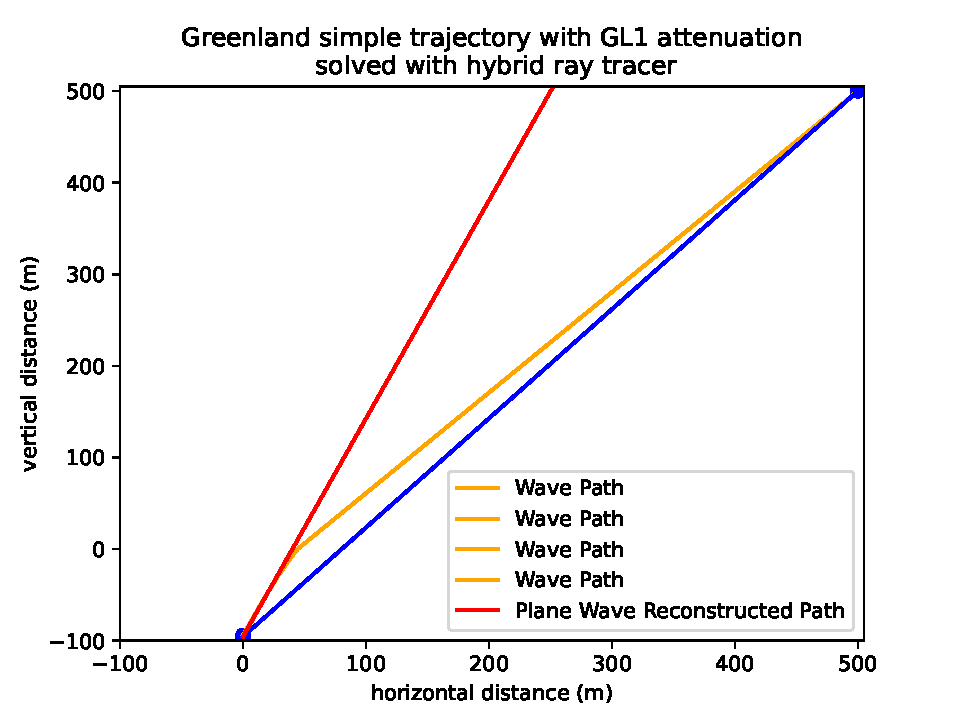
\includegraphics[width=0.7\textwidth]{WeatherBalloonPositionReconstruction.pdf}
	\caption{The balloon is too far away for a simple plane wave reconstruction, but using
  snells law at the surface might mitigate the problem.}
	\label{fig:WeatherBalloonPositionReconstruction}
\end{figure}
\section{Is the goal feasible?}
\label{sec:feasible}
In the example reconstruction illustrated in figure
\ref{fig:WeatherBalloonPositionReconstruction} the difference in angle between
direct to balloon and plane wave reconstruction is quite big
($\approx 65\%$) but as the balloon gets closer to the detector this reduces
significantly. As previously layed out, our goal is to find the local index of refraction n by using the
plane wave reconstruction with the recorded timing and the positional data from
the weather balloon.

Now let's ask ourselves the question, within which angles should the
weather balloon fly for the data to be useful?  The
further the weather balloon is away (in the x direction) the bigger the zenith
angle with the detector, the less accurate the plane wave reconstruction.  So
which angles are acceptable? Note that not only angle but also height will eventually
play a role in the accuracy, the angle however gives a good starting point.

To determine the accuracy we vary the position of the weather balloon in the x direction (keeping the
height constant at 500m), simulate the ray path to channels 0 to 3 and then fit n
both via the simple plane wave reconstruction method layed out in section \ref{seq:SimplePW} and
the one using snell's law layed out in section \ref{seq:SnellPW}.
We then compare the n's we have fitted  to the
one we know from the model at that position.  We quantify the discrepancy
between the fitted and known index of refraction via the
\textit{systematic error}:
\begin{equation}
  \varepsilon\ (\%) = \frac{n_\text{fit} - n_{\text{exact}}}{n_{\text{exact}}}
\end{equation}
Carrying this out we get figure
\ref{fig:EpsilonIFODirect}. Both the snell and simple plane wave method get
exponentially less accurate as the balloon moves further away.  If we wish the
systematic error to be within 1\% for the simple plane wave, the angle the
balloon makes with the middle of channels 0 to 3 needs to be less than 10°.
\begin{figure}
	\centering
	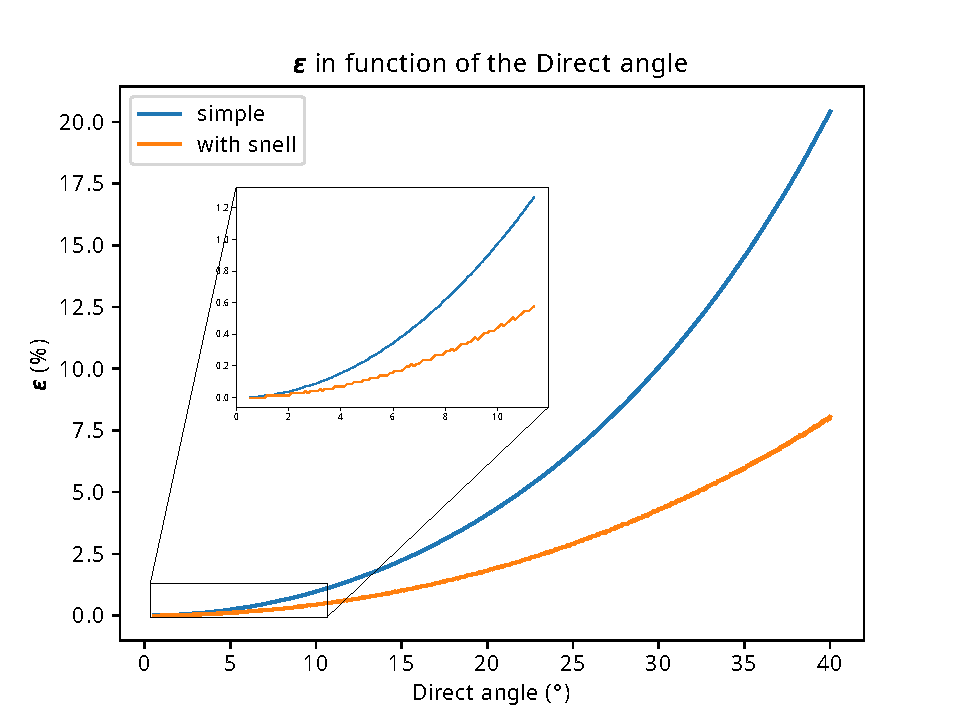
\includegraphics[width=0.8\textwidth]{EpsilonWithZoom.pdf}
	\caption{The accuracy of the plane wave reconstruction with the use of snell's law at the surface is more 
  accurate but the simple plane wave method's accuracy is sufficient to make reliable
predictions for angles less than 10°. For small angles the simple reconstruction is preferred as no ice 
parameters need to be assumed.}
	\label{fig:EpsilonIFODirect}
\end{figure}

Now can we actually find balloon passbys whom make an angle less than 10 degrees?
To figure this out we looped over all the balloon positions recorded over the summer of
2022, more particularly in the period 15/06/2022 - 30/09/2022
\footnote{The positional data of the weather balloons was obtained from the
\url{ftp1.esrl.noaa.gov} website using the rno-g-sonde script of the official
RNO-G github page.}, and recorded
the time intervals when they flew close enough.
To illustrate such a trajectory, an example path of a balloon passing close enough to a detector is shown in figure
\ref{fig:ExampleBalloonPathCrossing12}.
The data shown in appendices \ref{app:5Deg} and \ref{app:10Deg} respectively show $<5$° and $<10$° encounters.
\newpage
\begin{figure}
  \centering
	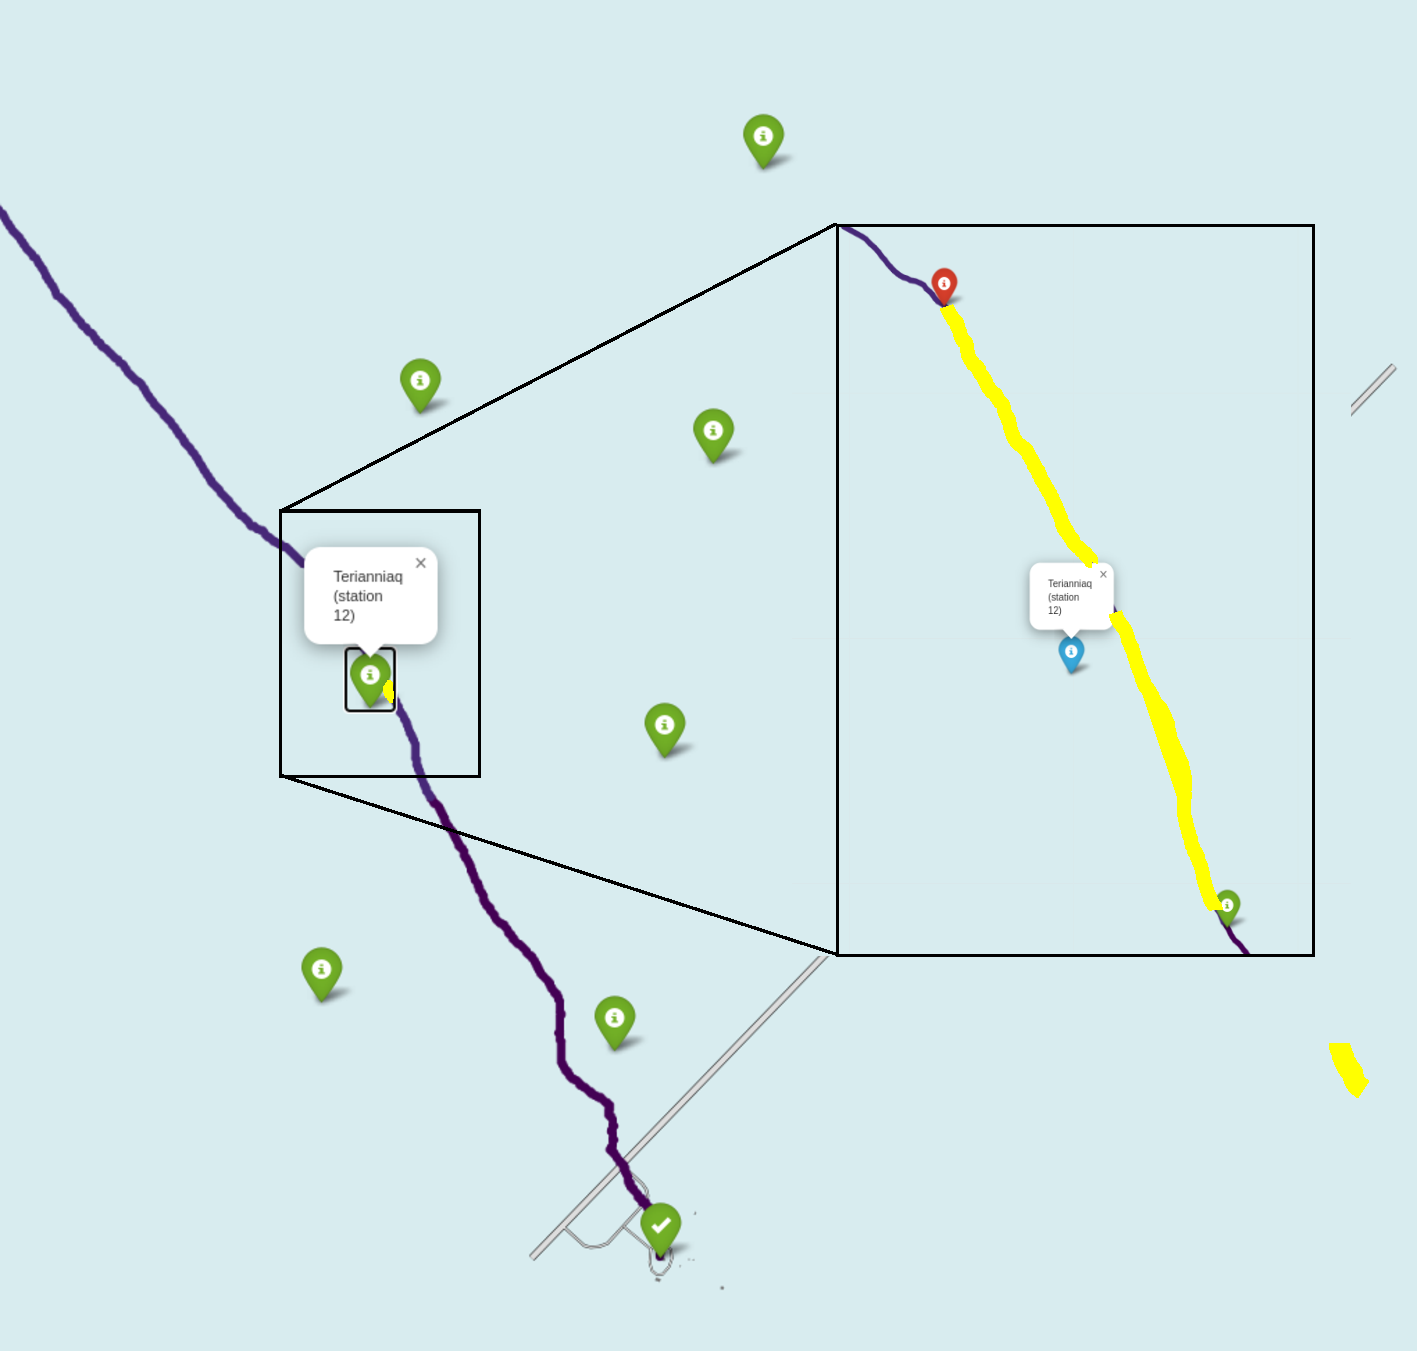
\includegraphics[width=0.5\textwidth]{BallonPathAllIllu.pdf}
  \caption{Path traced out by a weather balloon in purple released at 20/08/2022, in yellow you can see when it
  gets within 10° of detector 12. The green marks indicate the location of the various detectors.}
  \label{fig:ExampleBalloonPathCrossing12}
\end{figure}
\section{Fitting the index: Phased array}
Now that we know our goal to be feasible, let's analyze some data.  As we'll
start by just analyzing one event, let's take a reasonably good one for our analysis.

If we search in the DESY database
\footnote{\url{https://rnog-monitor.zeuthen.desy.de/}} within the calculated
time frames as listed in appendix \ref{app:5Deg} where the 403MHz signal coming from the
balloon is detected in the deep channels, the events of the 24th of July stands
out; at 23:21:53 the balloon gets quite close to detector 11 and shows a clear
403MHz signal at the phased array in channels 0,2 and 3, as shown for the
channels 2 and 3 in figure \ref{fig:freqs23}.

Now to calculate the differences in timing for this received signal, the code
we built for this is called FitN.py\cite{projects-mt}, 
let's go over the full code step by step:
\subsubsection{Spatial data}
The first part we'll need to concern ourselves with is determining the relative
positions of everything. The balloon data file and the time when the event took
place are given, from these two both the latitudinal and longitudinal position
and the elevation of the balloon at the given time are determined, which we convert
to ENU (x,y,z) coordinates as to be able to use them. 

The locations of the various stations have also been determined and can be found 
on the official RNO-G github under "analysis-tools". 

Now that we have both the position of our balloon and station, 
let's simplify the calculations by setting the detector as the
origin i.e our new balloon position will be
\begin{equation}
  \mathbf{r}_{bs} = \mathbf{r}_b- \mathbf{r}_s
\end{equation}
With the subscript b denoting "balloon" and s "station".
As we might want to plot this later, due to the cylindrical symmetry of the
ice, we can rotate the coordinates to get rid of our y-axis. We can do
this by defining the radius:
\begin{equation}
  r := \sqrt{x_{bs}^2 + y_{bs}^2}
\end{equation}
And redefining our relative position as
\begin{equation}
  \mathbf{r} = 
  \begin{bmatrix}
  r \\
  0 \\
  z_{bs}
  \end{bmatrix}
\end{equation}
We don't have the position of our individual channels yet, only of the station
itself. The relative position of these\footnote{relative to the detector} can
however also be obtained and as we chose our station to be the center of the
coordinate system, these relative positions are absolute positions of the
channels in our frame of reference.  Using these it thus doesn't matter where
the position of the station was defined.

\subsubsection{Signal analysis and initial guesses}
Now that we have the positions of both the balloon and the channels, let's
analyze the data. The data for a particular channel from a
recorded event (here event 12397 of run 1034) is stored in a channel object,
from this object we can get the recorded voltages and times during this event.
These recorded voltages can be Fourrier transformed to get the recorded
frequency spectrum.  We know that the signal sent out by the weather balloon is
a sine wave with a frequency of 403MHz; as the data is measured in nanoseconds
the frequency is:
\begin{equation}
	f = 403\text{MHz} = 403\times 10^{-3} \frac{1}{\text{ns}}
\end{equation}
The recorded spectrum of channels 2 and 3 is given in figure \ref{fig:freqs23}, for 
which we previously mentioned the spike at 0.403GHz.
\begin{figure}
	\begin{minipage}{0.49\textwidth}
		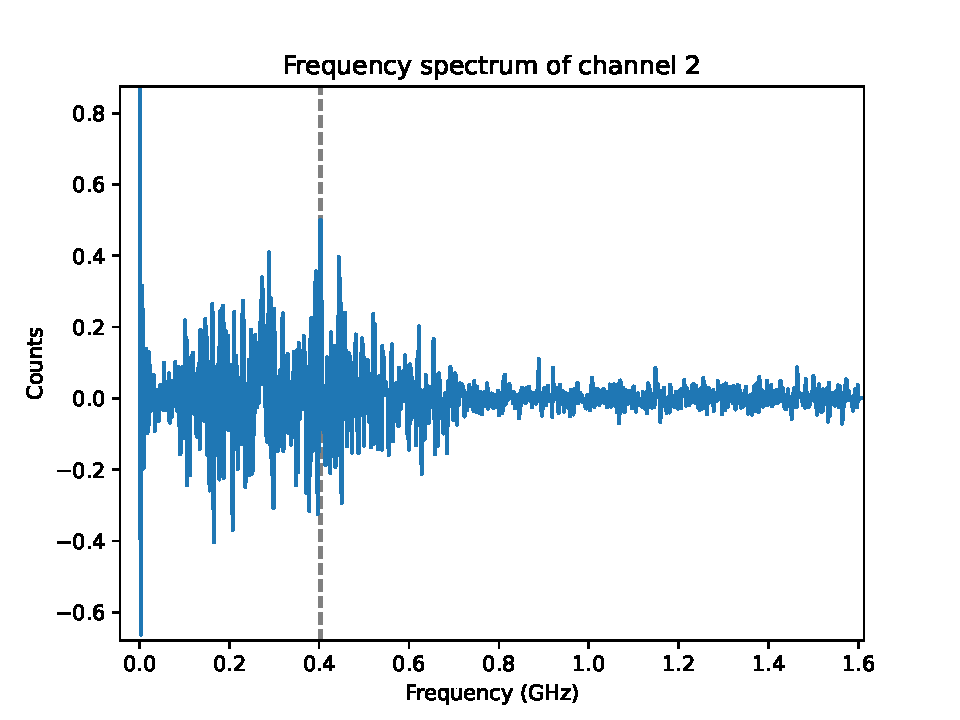
\includegraphics[width=\textwidth]{figures/2-freq.pdf}
	\end{minipage}
	\begin{minipage}{0.49\textwidth}
		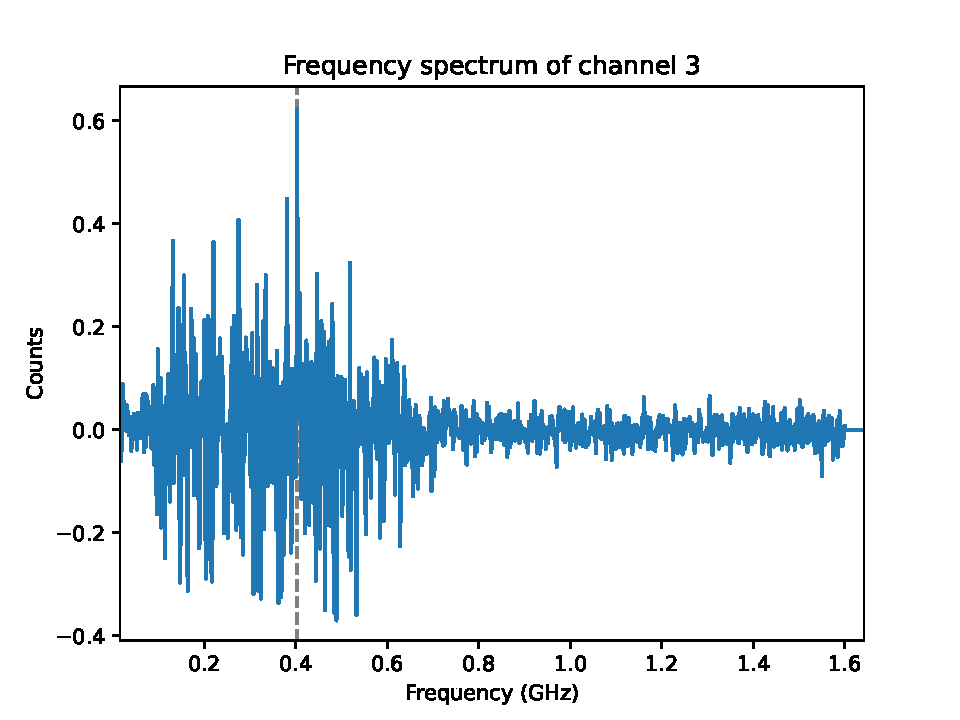
\includegraphics[width=\textwidth]{figures/3-freq.pdf}
	\end{minipage}
	\caption{recorded frequencies on detector 11 at 2022/07/24 23:21:53, clear spikes at 0.403GHz are visible}
	\label{fig:freqs23}
\end{figure}
Now note that on this figure it's shown that there are signals with frequencies
both below 0.15GHz and above 0.6GHz, these can be left out as the Vpol is
defined to be most responsive only in the range 0.15GHz to 0.6GHz
\cite{Aguilar_2021}. To filter out these frequencies we'll pass the signal trough a virtual
butterworth bandpass filter.

Now that we have filtered our data we'd also like to increase the accuracy in
timing, to this end we'll resample the signal\footnote{Resampling is the process of
changing the sampling rate of a discrete signal to obtain a new discrete
representation of the underlying continuous signal}. We'll upsample towards 10GHz
increasing our timely accuracy from 0.3125ns to 0.1ns, this is possible as the
full Nyquist-sampled waveforms are stored\cite{Allison_2019}.  As the timely accuracy
is now 0.1ns, the error on a time difference between channels is then 0.2ns. So
$\delta t_{ij}=0.2$ns as explained in section \ref{seq:SimplePW}.

After this cleaning of
our data (by filtering and upsampling) we have a voltage response with an example 
shown for channel 0 in figure \ref{fig:VoltageAfterFilter}, we wish to find a sine
wave coming from the weather balloon in this signal.
\begin{figure}
	\centering
	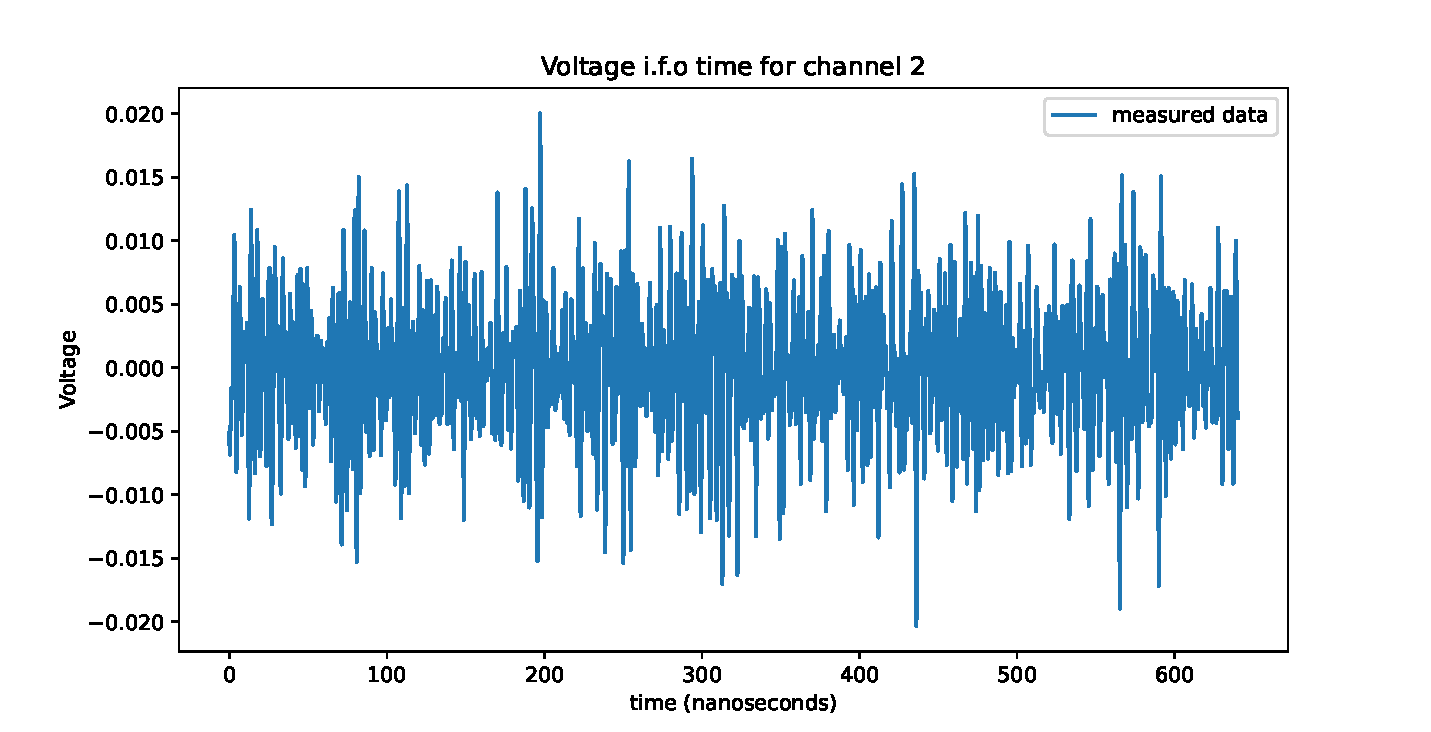
\includegraphics[width=\textwidth]{figures/VoltageAfterFilter.pdf}
	\caption{Recorded voltage i.f.o time in vpol antenna 2 after up sampling and passing through the butterworth filter, hereing we'll need to find a sinusoidal signal}
	\label{fig:VoltageAfterFilter}
\end{figure}
To find a sine wave herein, and thus find out the timing of our signal, we'll
make use of a method called \textit{cross correlation}, whereby we move a
template over our data, returning a high value if the data and template line up
and a low value if they don't.

We thus need a template to correlate with the data. The template we'll be choosing is
of course the sine function but it's important to notice that the channel has a
certain sampling rate, namely now after up sampling, 10GHz. 

Our template sine which we'll correlate to the data will also need to have this
sampling rate, meaning that it needs to be step wise defined with spaces of
0.1ns. Next we'll also need to give the sine a certain amplitude, as we don't
have a system for finding this let's assume an amplitude $A =0.007$ 
(this shouldn't impact the result).  Our template thus looks like this:
\begin{equation}
	\mathcal{S} = A\cdot\sin(\omega t) 
\end{equation}
with
\begin{equation}
	\omega = 2\pi f
\end{equation}
With f the frequency of the balloon signal, 0.403GHz and $t$ an array going
from 0 to $3/f$ as to be able to fit 3 periods, the
cross-correlation is done by moving the signal with steps of $\Delta t = 0.1$ns,
an illustrated of this procedure is shown in figure \ref{fig:SineCorrFull}. Mathematically this
amounts to evaluating\cite{Bracewell1966TheFT}:
\begin{equation}
  (f\star g)(\tau) \delequal \int_{-\infty}^\infty f(t)g(t+\tau)dt
\end{equation}
With f(t) the recorded signal and g(t) the sine wave template.

\begin{figure}
	\centering
	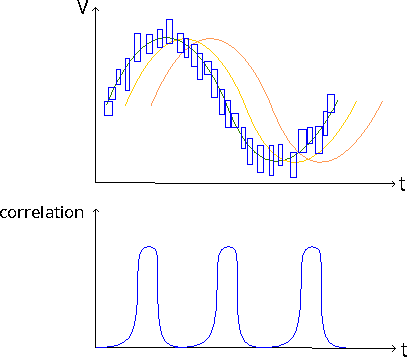
\includegraphics[width=0.8\textwidth]{figures/SineDataCorrFull.pdf}
	\caption{How correlating a sine with data leads to periodic peaks in the correlation function}
	\label{fig:SineCorrFull}
\end{figure}
In reality the data is a bit less perfect and after doing this correlation
procedure on the real data we get what's (partially) shown in figure \ref{fig:CorrCh2}.
\begin{figure}
	\centering
	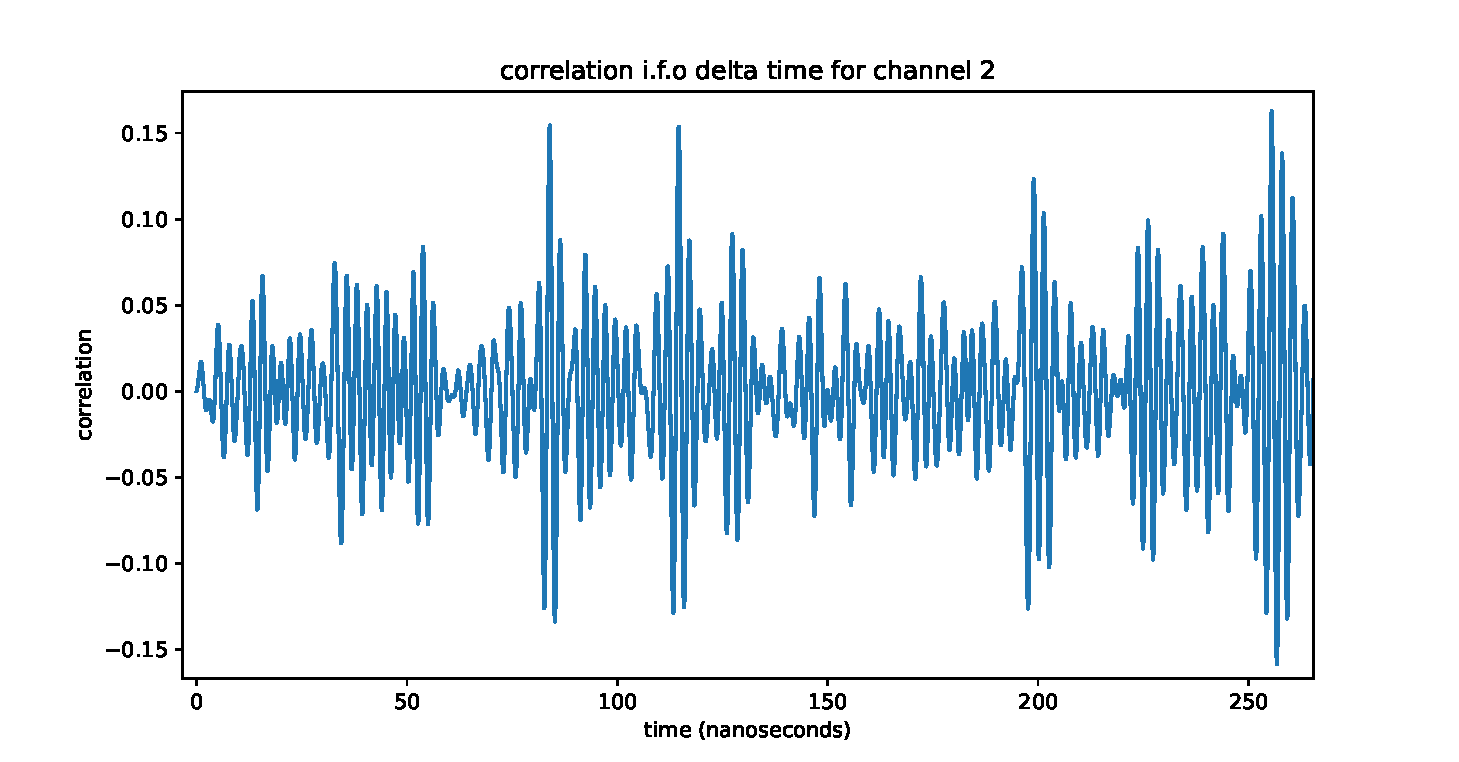
\includegraphics[width=\textwidth]{figures/CorrelationCh2.pdf}
	\caption{The correlation is less clear than in the illustration but still shows the periodicity of the sinusoidal signal}
	\label{fig:CorrCh2}
\end{figure}
Herein the peaks represent the maximal correlation, if we now do the same for
channel 3 we have two correlation functions, if we crosscorrelate these with
each other we'll get the difference in timing between the channels.  This is
easy to comprehend after taking a look at the illustration shown in figure
\ref{fig:IlluCorr}. 
\begin{figure}
  \centering
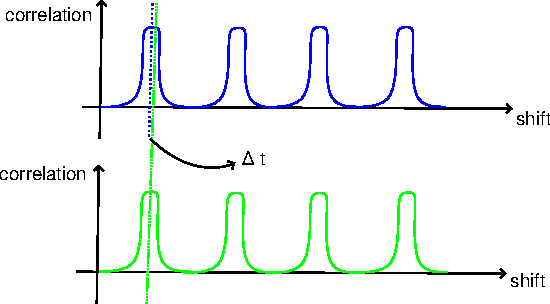
\includegraphics[width=0.8\textwidth]{figures/IlluCorr.pdf}
\caption{Crosscorrelating two crosscorrelated functions gives peaks at the differences in timing}
	\label{fig:IlluCorr}
\end{figure}
How this cross-correlation of cross-correlated functions then looks like is partially shown
in figure \ref{fig:CrossCrossCorr}, the negative offset is caused by us accounting for cable
delay. Note that multiple peak correlations are present. To find out which peak
is the actual one, and with that finding out what the difference in arrival time is which we
need to find our index of refraction, we'll need to analyse the physics of the problem.
\begin{figure}
  \centering
  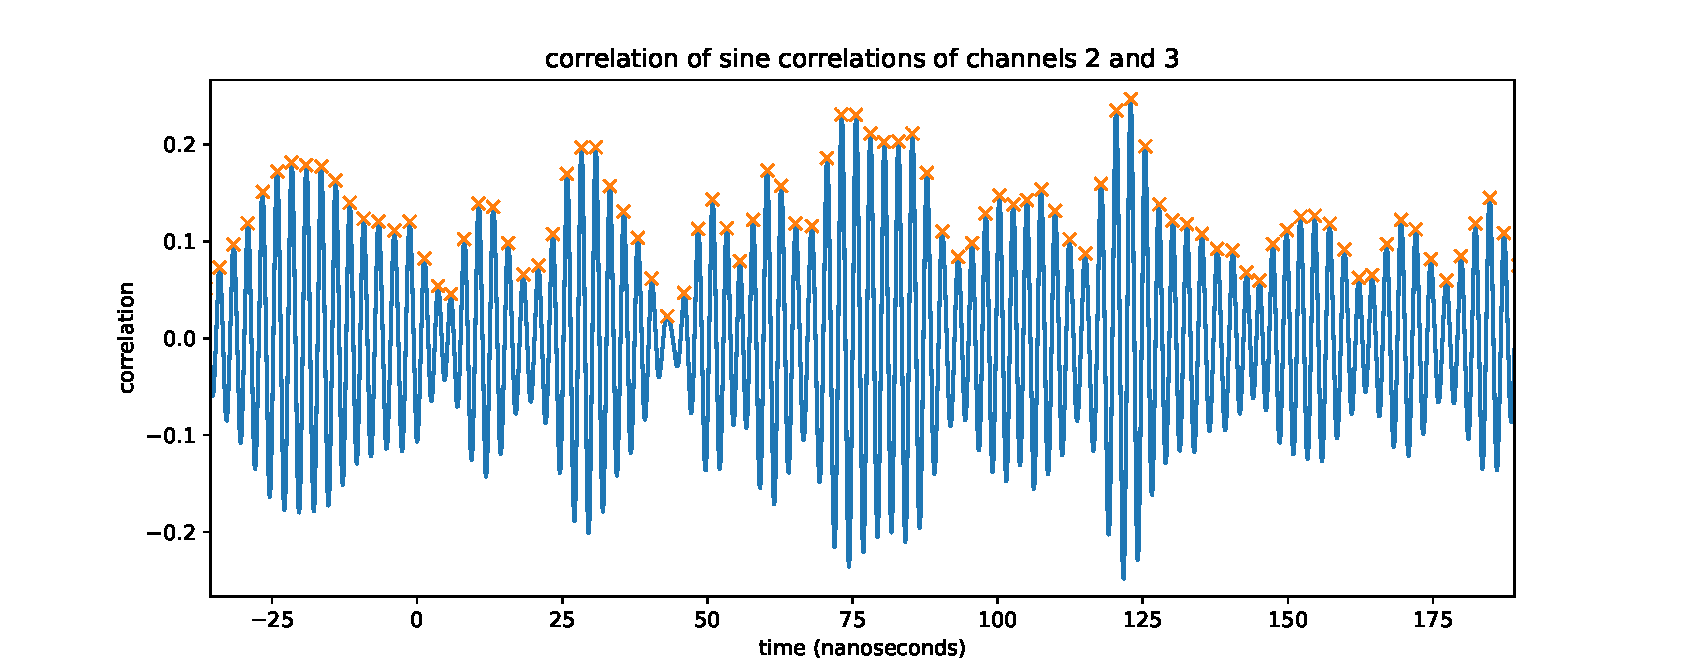
\includegraphics[width=\textwidth]{figures/CrossCrossCorr.pdf}
  \caption{Crosscorrelating two crosscorrelated functions gives peaks at the differences in timing}
	\label{fig:CrossCrossCorr}
\end{figure}

Our signal is sinusoidal with a frequency of 0.403GHz, locally our index of refraction should be around 1.7,
meaning that our wavelenght should be:
\begin{equation}
  \lambda = \frac{v}{f} = \frac{c}{nf} \approx 0.44m
\end{equation}
This wavelength is longer than the distance between the individual channels, meaning that if the top
of the sinusoidal wave gets detected in channel 2, then the sinusoidal wave gets detected in
channel 3 $\frac{1m}{0.44m} \approx 2.3$ wavelengths later. So we expect at least two peaks to 
have gone by until the same sinusoidal wave as in channel 2 gets detected in channel 3.
We thus have to search for the third peak (starting from t=0) in this case, similarly for detectors 0 and 3
which are spaced 3 meters apart we'll need to look at peak number $\lceil\frac{3m}{0.44m}\rceil = 7$.
And for completeness sake, for channels spaced 2 meters apart we'll need to look at peak 
$\lceil\frac{2m}{0.44m}\rceil = 5$. In reality however, it is easier to just simulate the time differences
and look in that neighbourhood.

\subsubsection{Fitting n and finding it's error}
Now that we have the differences in timing between the individual channels and their error, the
angle the balloon makes with the detector and the distance between the individual channels
all that's left to do is minimize function f as defined in equation \ref{eqn:PlaneWave} and
calculate the error. Doing the full procedure we get as a result:
\begin{center}
\begin{tabular}{||c c c c c c||}
 \hline
 Depth (m) & Station id & channels & Run:Event & n$_\text{exponential}$ & n$_\text{fit}$\\ [0.5ex]
 \hline\hline
 -94.518 & 11 & 0\&2\&3 & 1034:12397 & 1.7397 & 1.724 $\pm$ 0.014 $\pm$ 0.047 \\
 \hline
\end{tabular}
\end{center}
With the first error indicating the systematic error and the second error the error found through
error analysis. After varying both the positional and timely error it seems that the error on position is the biggest
contributing factor.

\section{Phased array and channels 5-7}
The event we'll now analyse is recorded in detector 21 at the 26th of July
11:18:41 and falls within the $<5$° mark, the balloon signal gets detected
by both the phased array and channels 5 to 7.

Channels 5 to 7 lie at a very interesting depth as, looking at 
the density versus depth data shown in figure \ref{fig:DensityMeasurements},
here (40-80m depth) the difference between the density measurements and the single
exponential model shows the largest deviations. 

As channels 5 to 7 are spaced quite far apart we can do the plane wave fitting 
for two channels at a time, still keeping the error quite small. The results are given below:
\begin{center}
\begin{tabular}{||c c c c c c||}
 \hline
 Depth (m) & Station id & channels & Run:Event & n$_\text{exponential}$ & n$_\text{fit}$\\ 
 \hline\hline
 -48.155 & 21 & 6\&7 & 1441:117 & 1.6400 & 1.632 $\pm$ 0.00128 $\pm$ 0.00472\\
 -58.38 & 21 & 5\&7 & 1441:117 & 1.6736 & 1.66632 $\pm$ 0.00226 $\pm$ 0.00233 \\
 -58.24 & 21 & 5\&6\&7 & 1441:117 & 1.67321 & 1.66553 $\pm$ 0.00167 $\pm$ 0.00350 \\
 -68.2 & 21 & 5\&6 & 1441:117 & 1.6983 & 1.69329 $\pm$0.00199$\pm$0.00460 \\
 -93.865 & 21 & 0\&1\&2\&3 & 1441:117 & 1.73896 & 1.71366$\pm$0.00287$\pm$0.05641\\
 \hline
\end{tabular}
\end{center}
\begin{figure}
	\centering
	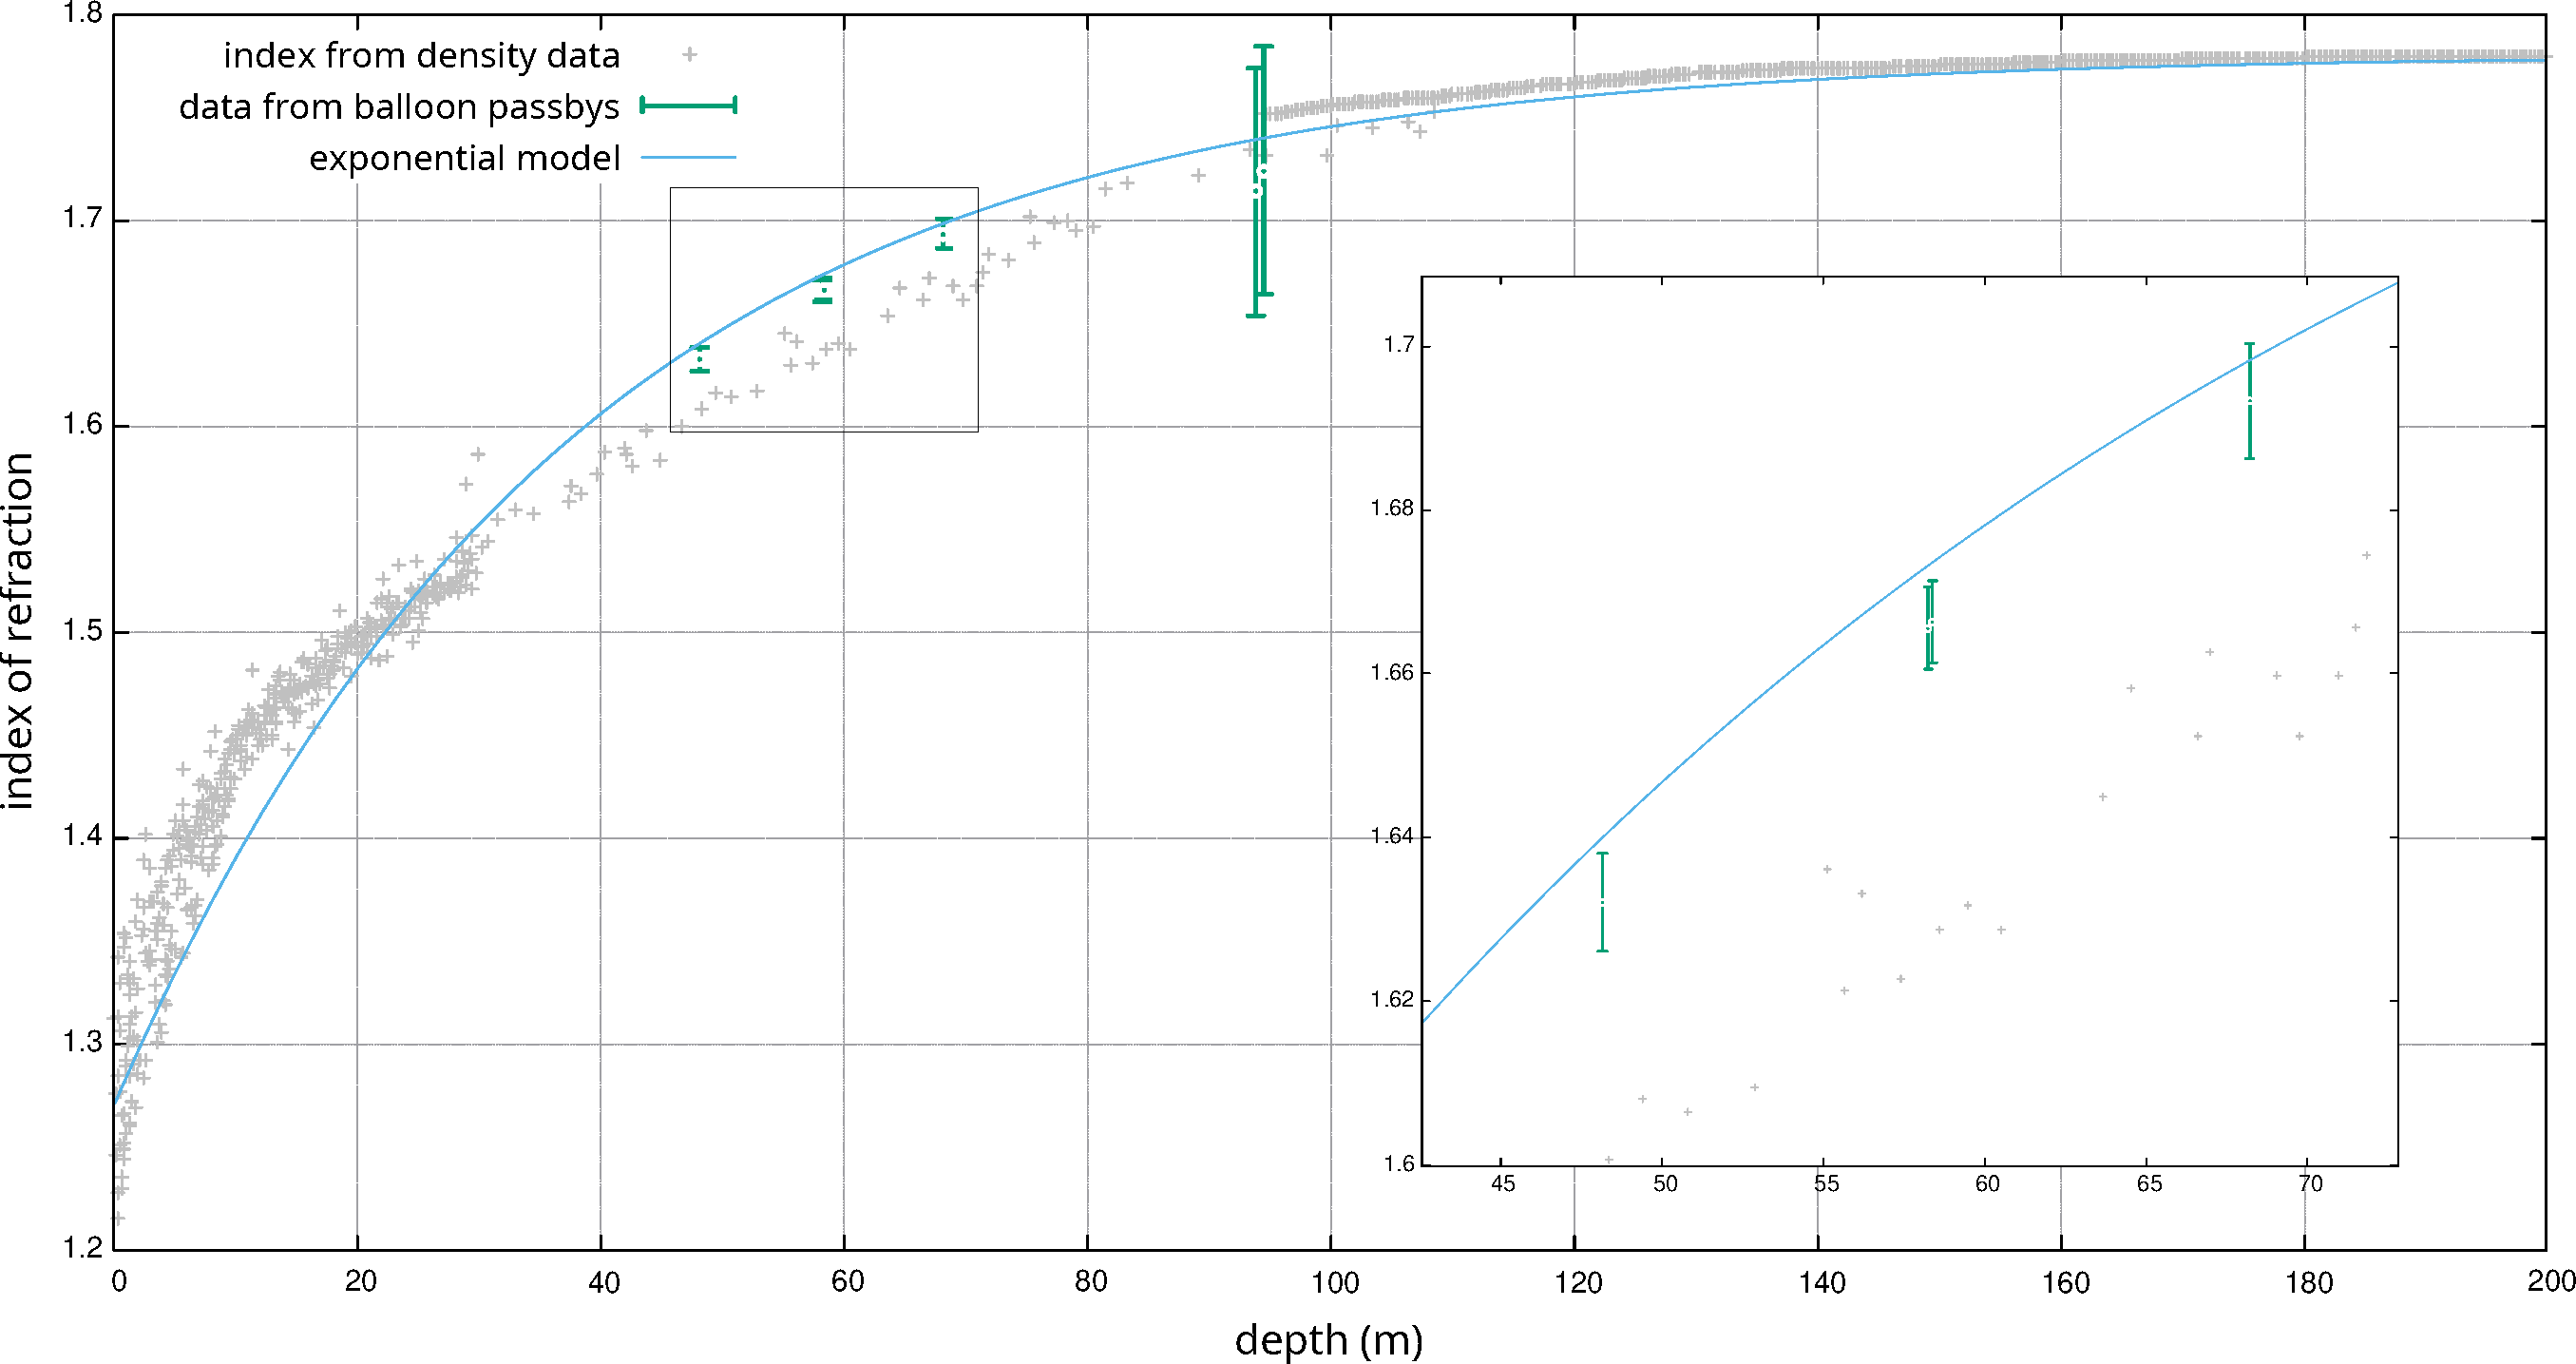
\includegraphics[width=\textwidth]{figures/ResultWithZoom.pdf}
  \caption{Even though the error bars are quite big, all values found within this chapter lie under the single exponential, 
    which is especially clear at the phased array depths where the measurements
    are below both the exponential model and the data from the converted densities}
	\label{fig:Results}
\end{figure}
\section{Evaluation of the results}
All the fits that were found are visually shown in figure \ref{fig:Results},  together
with the index found by converting the density data through the linear index-density relation
($n(z) \approx 1 + 0.845\rho(z)$) and the exponential model\footnote{A bigger version can also be found in appendix \ref{app:ExtraFigures}}.
Note that all of the indices that have been found have a value below the
exponential model's, more closely to the converted density data.
Even though the error is quite big these results could raise some
suspision on the validity of the exponential model and might indicate
that it's needed to measure the whole index-depth profile.

Now note that the measurements on depths 40-80m don't fully agree with the density data, 
this could be caused by one of the following reasons:
\begin{itemize}
	\item The density measurements aren't accurate enough
	\item The index isn't fully linear at every depth
	\item The fit isn't accurate enough and thus the error bars are underestimated
\end{itemize}
The density measurements do actually show quite a lot of spread for
nearly the same values so there might be a problem there. There are
also not that many recorded measurements in the 40-100m region and no reported
uncertainties which makes the data less trustworthy.  

As for the linearity relation, it has been extensively studied in the literature
\cite{KOVACS1995245} and there seem to be multiple relationships reported,
all however were linear. Another possible relation is e.g
\begin{equation}
  n(z) \approx 1 + 0.77\rho(z)
\end{equation}
How our data correlates with this relation is shown in figure
\ref{fig:ResultsOtherLinear}, but this doesn't seem to heavily impact the
distance from the density converted data and our measurements.

Lastly as channels 5-7 are spaced quite far apart, the plane wave reconstruction
might not be fully viable and the assumption that the incoming angle is the same for
all channels not fully correct. But as the balloon is really close during this event
we think that this contribution is negligable and the results should be somewhat viable.

It might thus be needed to measure the index-depth relation directly and so
obtain an experiments-based ice model.
